%!TEX root = ./main.tex

\section[Bench \& Standards]{On the Bench, and On the Clock}

% SECTION TIMING: 64:00--70:00 (4 frames).
% TEACHING NOTE: after forty minutes of optimisation, the point of this section is that
% somebody actually built it -- and that the measured numbers are much coarser than the
% simulated ones. Say that out loud on the results frame.

\begin{frame}{Somebody actually built one}
  \vspace{0.3em}
  \begin{columns}[T,onlytextwidth]
    \column{0.42\textwidth}
      \centering
      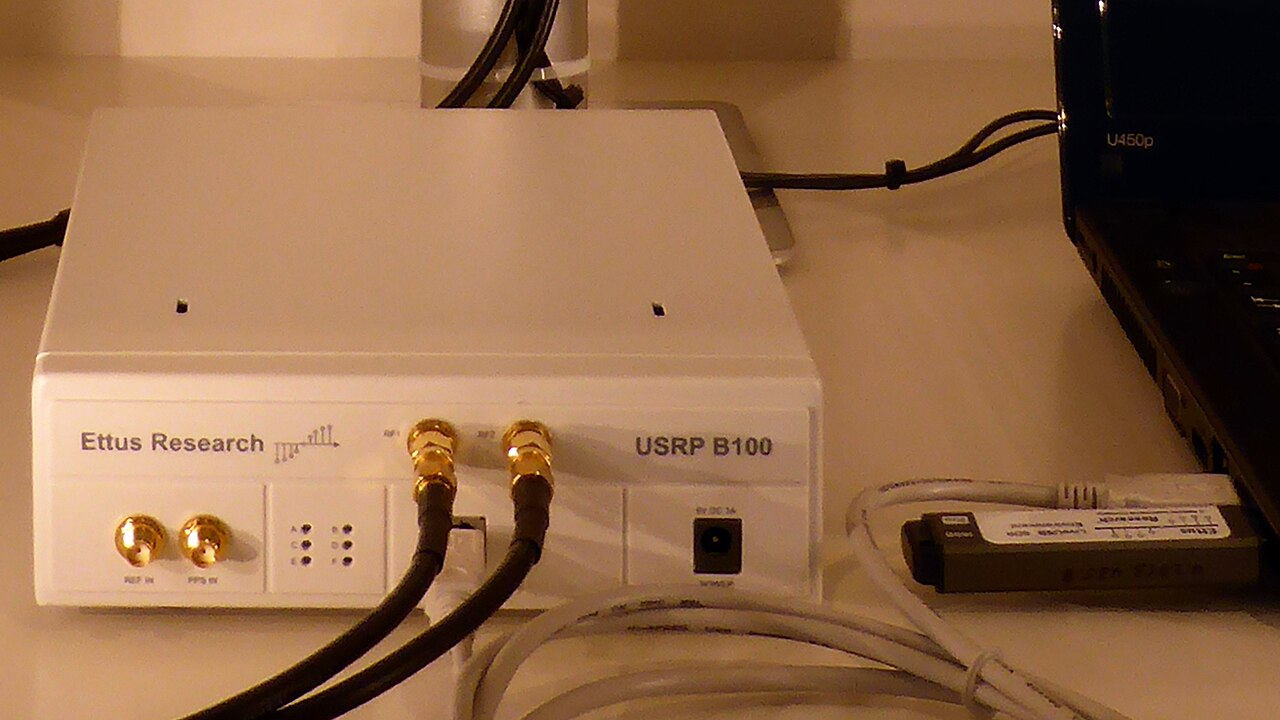
\includegraphics[width=\linewidth]{figure/isac/usrp_b100.jpg}
      \source{https://commons.wikimedia.org/wiki/File:USRP_B100_(crop).jpg}{USRP software-defined radio (illustrative)}
    \column{0.54\textwidth}
      \small
      \begin{itemize}\itemsep4pt
        \item A host PC drives the bench.
        \item An FPGA steers the surface.
        \item USRP plus a converter.
        \item Transmit on the surface.
        \item Receive on a horn antenna.
        \item A target module fakes echoes.
      \end{itemize}
  \end{columns}

  \glossline{RHS = Reconfigurable Holographic Surface \quad
    USRP = Universal Software Radio Peripheral \quad
    FPGA = Field-Programmable Gate Array}

  \vspace{0.2em}
  \takeaway{Two main lobes: one aimed at a user, one at a target.\\One aperture, at the same time.}
\end{frame}

\begin{frame}{Inside the chamber}
  \begin{columns}[T,onlytextwidth]
    \column{0.44\textwidth}
      \centering
      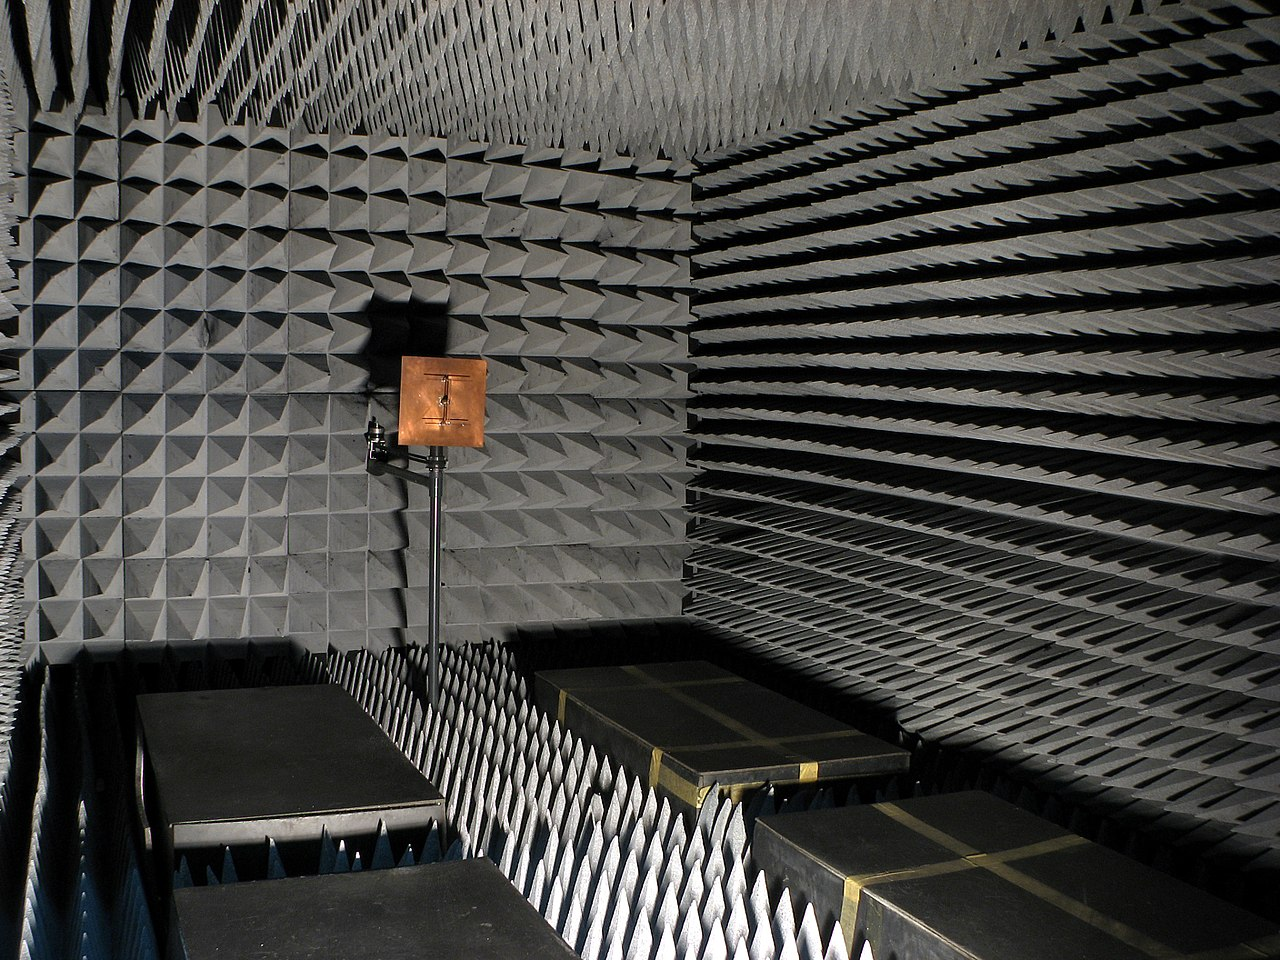
\includegraphics[width=\linewidth]{figure/isac/anechoic_chamber.jpg}
      \source{https://commons.wikimedia.org/wiki/File:Radio-frequency-anechoic-chamber-HDR-0a.jpg}{RF anechoic chamber, Democritus University of Thrace}
    \column{0.52\textwidth}
      \small
      \begin{itemize}\itemsep5pt
        \item Chamber about 4\,m cubed.
        \item Lobe steered to $-50^\circ$, $0^\circ$, $20^\circ$.
        \item Estimated range tracks truth.
        \item Second lobe carries live data.
      \end{itemize}
  \end{columns}

  \vspace{0.3em}
  \qa{Why prove it in an anechoic chamber first?}
     {Because the chamber removes every echo you did not create. If sensing fails
      there, the waveform is wrong; if it fails outdoors, the world is the
      variable.}

  \source{https://ieeexplore.ieee.org/document/10681896}{IEEE/CIC ICCC 2024, Best Demo Award}
\end{frame}

% ACCURACY NOTE: the outdoor and indoor numbers below are the demo's own measured
% accuracies. 15 degrees of angular accuracy is coarse -- that is the honest point of
% the frame. Do not soften it.
\begin{frame}{Measured numbers are humbler}
  \vspace{0.5em}
  \begin{columns}[T,onlytextwidth]
    \column{0.47\textwidth}
      \large\textbf{\textcolor{ranblue}{Range, outdoors}}

      \vspace{0.5em}
      \small
      \begin{itemize}\itemsep4pt
        \item Target: a metal plate
        \item Span: 4--21\,m
        \item Accuracy: about 0.425\,m
      \end{itemize}
    \column{0.47\textwidth}
      \large\textbf{\textcolor{coreorange}{Angle, indoors}}

      \vspace{0.5em}
      \small
      \begin{itemize}\itemsep4pt
        \item Same metal plate
        \item Span: $-60^\circ$ to $+60^\circ$
        \item Accuracy: about $15^\circ$
      \end{itemize}
  \end{columns}

  \vspace{0.9em}
  \ask{Half a metre and fifteen degrees.\\Which applications does that already serve?}
\end{frame}

% ACCURACY NOTE: this timeline is the SPEAKER'S PROJECTION, not a published schedule.
% 3GPP Release 19 ISAC study work is real; Release 21 dates and "ITU adoption of ISAC in
% IMT-2030" phrasing beyond M.2160 are forecasts. Present it as a forecast.
\begin{frame}{The clock, as of this talk}
  \vspace{0.6em}
  \centering
  \begin{tikzpicture}[scale=0.9,transform shape,
      ph/.style={draw=ranblue,fill=blue!5,rounded corners=3pt,
        minimum width=1.85cm,minimum height=0.8cm,align=center,font=\scriptsize\bfseries},
      note/.style={align=center,font=\scriptsize,text width=2.35cm}]
    \node[ph] (a) at (0,0) {2020--23};
    \node[ph] (b) at (2.45,0) {2024--26};
    \node[ph] (c) at (4.9,0) {2027--28};
    \node[ph,draw=coreorange,fill=orange!7] (d) at (7.35,0) {2029--30};
    \node[ph,draw=softgreen,fill=green!5] (e) at (9.8,0) {2031+};
    \foreach \x/\y in {a/b,b/c,c/d,d/e} \draw[flow] (\x) -- (\y);
    \node[note] at (0,-1.3) {concept and use cases};
    \node[note] at (2.45,-1.3) {3GPP Rel-19; trials};
    \node[note] at (4.9,-1.3) {spectrum policy};
    \node[note] at (7.35,-1.3) {specs and certification};
    \node[note] at (9.8,-1.3) {commercial rollout};
  \end{tikzpicture}

  \vspace{1.4em}
  {\scriptsize\textcolor{softgray}{The 2020--2026 columns describe work that has
   happened. Everything from 2027 rightward is a forecast made in this talk, not a
   published schedule.}\par}

  \vspace{0.4em}
  \takeaway{Standardisation is where the tradeoff stops being a curve\\and starts being a number somebody must certify.}
\end{frame}
